\documentclass[11pt]{article}

%====================================================
% PACKAGES
%====================================================

\usepackage[a4paper,margin=0.5in]{geometry}

\usepackage{amsmath,amssymb}
\usepackage{graphicx}
\usepackage{array}
\usepackage{multicol}
\usepackage{xcolor}

\usepackage{tikz}
\usetikzlibrary{decorations.pathmorphing}

\usepackage{tcolorbox}

%====================================================
% PAGE SETTINGS
%====================================================

\pagestyle{plain}

\setlength{\multicolsep}{6pt}

%====================================================
% DOCUMENT
%====================================================

\begin{document}

%====================================================
% TITLE
%====================================================

\begin{center}
    {\Huge \textbf{Algebra 1 -- Transformations Worksheet}}
\end{center}

\vspace{0.2cm}

\begin{center}
\Large
Visualizing Transformations Through Motion, Springs, and Mirrors
\end{center}

\vspace{0.4cm}

\noindent
\textbf{Name:} \underline{\hspace{5cm}}
\hfill
\textbf{Date:} \underline{\hspace{3cm}}

\vspace{0.5cm}

%====================================================
% LEARNING OBJECTIVES
%====================================================

\begin{tcolorbox}[
colback=gray!5,
colframe=black,
title=\Large Learning Goals
]

By the end of this worksheet, students should be able to:

\begin{itemize}

\item Translate points on the coordinate plane

\item Understand horizontal and vertical stretch/shrink visually

\item Identify how coordinates change during transformations

\item Reflect figures across lines

\item Explain transformations conceptually

\end{itemize}

\end{tcolorbox}

\vspace{0.5cm}

%====================================================
% VOCABULARY
%====================================================

\begin{tcolorbox}[
colback=yellow!5,
colframe=orange,
title=\Large Transformation Vocabulary
]

\begin{itemize}

\item \textbf{Translation} = slide

\item \textbf{Reflection} = flip like a mirror

\item \textbf{Stretch} = move farther from an axis

\item \textbf{Shrink} = move closer to an axis

\end{itemize}

\end{tcolorbox}

\vspace{0.5cm}

%====================================================
% SECTION A
%====================================================

\begin{tcolorbox}[
colback=blue!3,
colframe=blue,
title=\Large A. Warm Up -- Directions from a Point
]

Start from the point $P$. Find the new point after moving in the given direction.

\vspace{0.3cm}

\[
\text{Left 1} \rightarrow (x-1,y)
\qquad
\text{Right 2} \rightarrow (x+2,y)
\]

\[
\text{Up 3} \rightarrow (x,y+3)
\qquad
\text{Down 4} \rightarrow (x,y-4)
\]

\vspace{0.4cm}

\textbf{Example: } $P(2,1)$

\begin{center}

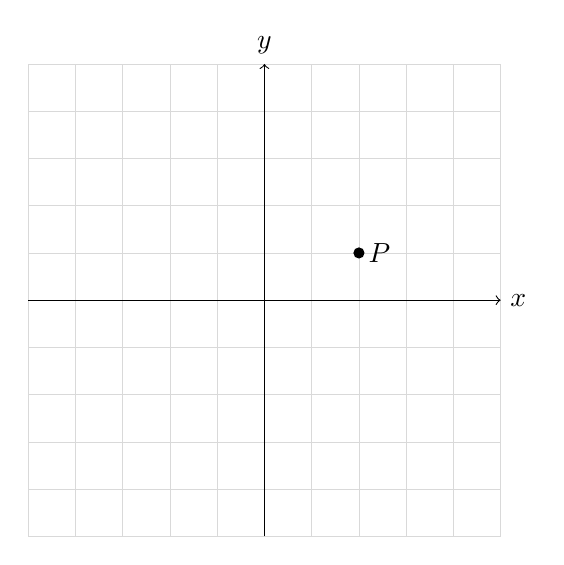
\begin{tikzpicture}[scale=0.6]

\draw[step=1cm,gray!30,very thin] (-5,-5) grid (5,5);

\draw[->] (-5,0)--(5,0) node[right]{$x$};

\draw[->] (0,-5)--(0,5) node[above]{$y$};

\filldraw[black] (2,1) circle (3pt);

\node[right] at (2,1) {$P$};

\end{tikzpicture}

\end{center}

\vspace{0.2cm}

\begin{itemize}

\item Left 1: \underline{\hspace{3cm}}

\item Right 2: \underline{\hspace{3cm}}

\item Up 3: \underline{\hspace{3cm}}

\item Down 4: \underline{\hspace{3cm}}

\end{itemize}

\vspace{0.3cm}

\begin{center}

\fbox{
\parbox{0.85\linewidth}{
\textbf{Key Idea:}
Moving left/right changes the x-coordinate.
Moving up/down changes the y-coordinate.
}
}

\end{center}

\end{tcolorbox}

\vspace{0.5cm}

%====================================================
% SECTION B
%====================================================

\begin{tcolorbox}[
colback=green!3,
colframe=green!50!black,
title=\Large B. Stretch / Shrink (The Spring Model)
]

Think of a spring attached to an axis.

\vspace{0.3cm}

\begin{itemize}

\item Horizontal stretch/shrink:
spring attached to the \textbf{y-axis}

\item Vertical stretch/shrink:
spring attached to the \textbf{x-axis}

\end{itemize}

\vspace{0.5cm}

\hrule

\vspace{0.5cm}

%====================================================
% HORIZONTAL
%====================================================

{\Large \textbf{Horizontal Stretch \& Shrink}}

\vspace{0.2cm}

\[
(x,y)\rightarrow(kx,y)
\]

\vspace{0.4cm}

\small

\begin{multicols}{3}

%----------------------------------------------------
% ORIGINAL
%----------------------------------------------------

\begin{center}

\textbf{Original ($k=1$)}

\vspace{0.2cm}

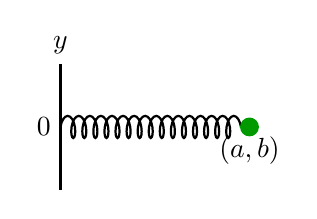
\begin{tikzpicture}[scale=0.8]

\draw[thick] (0,-1)--(0,1);

\node[above] at (0,1) {$y$};

\node[left] at (0,0) {$0$};

\draw[
decorate,
decoration={
coil,
aspect=0.4,
segment length=4pt,
amplitude=4pt
},
thick
]
(0,0)--(3,0);

\filldraw[green!60!black] (3,0) circle (4pt);

\node[below] at (3,0) {$(a,b)$};

\end{tikzpicture}

\end{center}

\columnbreak

%----------------------------------------------------
% STRETCH
%----------------------------------------------------

\begin{center}

\textbf{Stretch ($k>1$)}

\vspace{0.2cm}

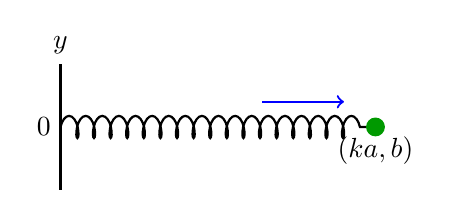
\begin{tikzpicture}[scale=0.8]

\draw[thick] (0,-1)--(0,1);

\node[above] at (0,1) {$y$};

\node[left] at (0,0) {$0$};

\draw[
decorate,
decoration={
coil,
aspect=0.4,
segment length=6pt,
amplitude=4pt
},
thick
]
(0,0)--(5,0);

\draw[->,thick,blue] (3.2,0.4)--(4.5,0.4);

\filldraw[green!60!black] (5,0) circle (4pt);

\node[below] at (5,0) {$(ka,b)$};

\end{tikzpicture}

\end{center}

\columnbreak

%----------------------------------------------------
% SHRINK
%----------------------------------------------------

\begin{center}

\textbf{Shrink ($0<k<1$)}

\vspace{0.2cm}

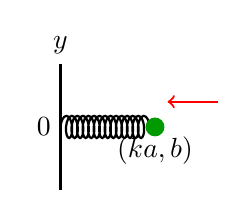
\begin{tikzpicture}[scale=0.8]

\draw[thick] (0,-1)--(0,1);

\node[above] at (0,1) {$y$};

\node[left] at (0,0) {$0$};

\draw[
decorate,
decoration={
coil,
aspect=0.4,
segment length=2pt,
amplitude=4pt
},
thick
]
(0,0)--(1.5,0);

\draw[->,thick,red] (2.5,0.4)--(1.7,0.4);

\filldraw[green!60!black] (1.5,0) circle (4pt);

\node[below] at (1.5,0) {$(ka,b)$};

\end{tikzpicture}

\end{center}

\end{multicols}

\normalsize

\vspace{0.4cm}

\begin{center}

\fbox{
\parbox{0.85\linewidth}{
\textbf{Key Idea:}
Horizontal stretch changes the distance from the y-axis.
The y-coordinate stays the same.
}
}

\end{center}

\vspace{0.3cm}

\textbf{Think About It:}

Why does the y-coordinate stay the same?

\vspace{0.6cm}

\hrule

\vspace{0.6cm}

%====================================================
% VERTICAL
%====================================================

{\Large \textbf{Vertical Stretch \& Shrink}}

\vspace{0.2cm}

\[
(x,y)\rightarrow(x,ky)
\]

\vspace{0.4cm}

\small

\begin{multicols}{3}

%----------------------------------------------------
% ORIGINAL
%----------------------------------------------------

\begin{center}

\textbf{Original ($k=1$)}

\vspace{0.2cm}

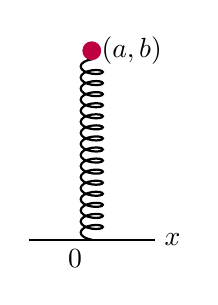
\begin{tikzpicture}[scale=0.8]

\draw[thick] (-1,0)--(1,0);

\node[right] at (1,0) {$x$};

\node[below left] at (0,0) {$0$};

\draw[
decorate,
decoration={
coil,
aspect=0.4,
segment length=4pt,
amplitude=4pt
},
thick
]
(0,0)--(0,3);

\filldraw[purple] (0,3) circle (4pt);

\node[right] at (0,3) {$(a,b)$};

\end{tikzpicture}

\end{center}

\columnbreak

%----------------------------------------------------
% STRETCH
%----------------------------------------------------

\begin{center}

\textbf{Stretch ($k>1$)}

\vspace{0.2cm}

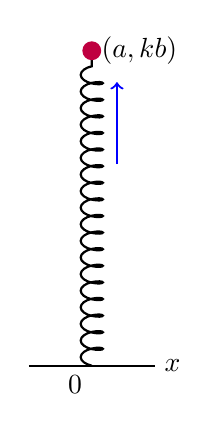
\begin{tikzpicture}[scale=0.8]

\draw[thick] (-1,0)--(1,0);

\node[right] at (1,0) {$x$};

\node[below left] at (0,0) {$0$};

\draw[
decorate,
decoration={
coil,
aspect=0.4,
segment length=6pt,
amplitude=4pt
},
thick
]
(0,0)--(0,5);

\draw[->,thick,blue] (0.4,3.2)--(0.4,4.5);

\filldraw[purple] (0,5) circle (4pt);

\node[right] at (0,5) {$(a,kb)$};

\end{tikzpicture}

\end{center}

\columnbreak

%----------------------------------------------------
% SHRINK
%----------------------------------------------------

\begin{center}

\textbf{Shrink ($0<k<1$)}

\vspace{0.2cm}

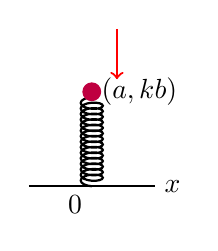
\begin{tikzpicture}[scale=0.8]

\draw[thick] (-1,0)--(1,0);

\node[right] at (1,0) {$x$};

\node[below left] at (0,0) {$0$};

\draw[
decorate,
decoration={
coil,
aspect=0.4,
segment length=2pt,
amplitude=4pt
},
thick
]
(0,0)--(0,1.5);

\draw[->,thick,red] (0.4,2.5)--(0.4,1.7);

\filldraw[purple] (0,1.5) circle (4pt);

\node[right] at (0,1.5) {$(a,kb)$};

\end{tikzpicture}

\end{center}

\end{multicols}

\normalsize

\vspace{0.4cm}

\begin{center}

\fbox{
\parbox{0.85\linewidth}{
\textbf{Key Idea:}
Vertical stretch changes the distance from the x-axis.
The x-coordinate stays the same.
}
}

\end{center}

\vspace{0.3cm}

\textbf{Think About It:}

Why does the x-coordinate stay the same?

\end{tcolorbox}

\vspace{0.5cm}

%====================================================
% SECTION C
%====================================================

\begin{tcolorbox}[
colback=purple!3,
colframe=purple,
title=\Large C. Reflections
]

\begin{multicols}{2}

\begin{align*}
\text{Over x-axis:} \quad
(x,y) &\rightarrow (x,-y)
\\
\\
\text{Over y-axis:} \quad
(x,y) &\rightarrow (-x,y)
\\
\\
\text{Over } y=x: \quad
(x,y) &\rightarrow (y,x)
\\
\\
\text{Over } y=-x: \quad
(x,y) &\rightarrow (-y,-x)
\end{align*}

\columnbreak

\begin{center}

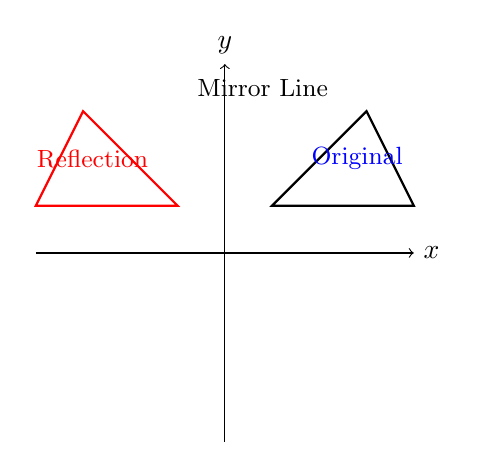
\begin{tikzpicture}[scale=0.6]

\draw[->] (-4,0)--(4,0) node[right]{$x$};

\draw[->] (0,-4)--(0,4) node[above]{$y$};

\draw[dashed] (0,-4)--(0,4);

\node at (0.8,3.5) {\small Mirror Line};

\draw[thick]
(1,1)--(3,3)--(4,1)--cycle;

\node[blue] at (2.8,2) {\small Original};

\draw[red,thick]
(-1,1)--(-3,3)--(-4,1)--cycle;

\node[red] at (-2.8,2) {\small Reflection};

\end{tikzpicture}

\end{center}

\end{multicols}

\vspace{0.4cm}

\begin{center}

\fbox{
\parbox{0.85\linewidth}{
\textbf{Key Idea:}
Reflections flip a figure across a line like a mirror.
}
}

\end{center}

\end{tcolorbox}

\vspace{0.5cm}

%====================================================
% FUNCTION CONNECTION
%====================================================

\begin{tcolorbox}[
colback=cyan!5,
colframe=cyan!60!black,
title=\Large D. Connection to Functions
]

Transformations also appear in functions.

\vspace{0.3cm}

\[
f(x)+3
\]

moves a graph up 3 units.

\vspace{0.3cm}

\[
-f(x)
\]

reflects a graph over the x-axis.

\vspace{0.3cm}

\[
f\left(\frac{x}{2}\right)
\]

creates a horizontal stretch.

\vspace{0.3cm}

\[
2f(x)
\]

creates a vertical stretch.

\end{tcolorbox}

\vspace{0.5cm}

%====================================================
% SELF REFLECTION
%====================================================

\begin{tcolorbox}[
colback=yellow!5,
colframe=orange,
title=\Large Self Reflection
]

\begin{itemize}

\item Which transformation was easiest for you?

\vspace{0.5cm}

\item Which transformation was hardest?

\vspace{0.5cm}

\item What does ``stretch'' really mean geometrically?

\vspace{0.5cm}

\item What does ``reflection'' really mean visually?

\vspace{0.5cm}

\item What is one mistake you should avoid next time?

\vspace{0.5cm}

\end{itemize}

\end{tcolorbox}

\vspace{0.5cm}

%====================================================
% FINAL MESSAGE
%====================================================

\begin{center}

{\LARGE
\textbf{
Remember:
Transformations change position, size, or direction!
}
}

\end{center}

\end{document}
